% Digital Logic Report Template
% Created: 2019-09-13, John Miller

%==========================================================
%=========== Document Setup  ==============================

% Formatting defined by class file
\documentclass[11pt]{article}

% ---- Document formatting ----
\usepackage[margin=1in]{geometry}	% Narrower margins
\usepackage{booktabs}				% Nice formatting of tables
\usepackage{graphicx}				% Ability to include graphics

%\setlength\parindent{0pt}	% Do not indent first line of paragraphs 
\usepackage[parfill]{parskip}		% Line space b/w paragraphs
%	parfill option prevents last line of pgrph from being fully justified

% Parskip package adds too much space around titles, fix with this
\RequirePackage{titlesec}
\titlespacing\section{0pt}{8pt plus 4pt minus 2pt}{3pt plus 2pt minus 2pt}
\titlespacing\subsection{0pt}{4pt plus 4pt minus 2pt}{-2pt plus 2pt minus 2pt}
\titlespacing\subsubsection{0pt}{2pt plus 4pt minus 2pt}{-6pt plus 2pt minus 2pt}

% ---- Hyperlinks ----
\usepackage[colorlinks=true,urlcolor=blue]{hyperref}	% For URL's. Automatically links internal references.

% ---- Code listings ----
\usepackage{listings} 					% Nice code layout and inclusion
\usepackage[usenames,dvipsnames]{xcolor}	% Colors (needs to be defined before using colors)

% Define custom colors for listings
\definecolor{listinggray}{gray}{0.98}		% Listings background color
\definecolor{rulegray}{gray}{0.7}			% Listings rule/frame color

% Style for Verilog
\lstdefinestyle{Verilog}{
	language=Verilog,					% Verilog
	backgroundcolor=\color{listinggray},	% light gray background
	rulecolor=\color{blue}, 			% blue frame lines
	frame=tb,							% lines above & below
	linewidth=\columnwidth, 			% set line width
	basicstyle=\small\ttfamily,	% basic font style that is used for the code	
	breaklines=true, 					% allow breaking across columns/pages
	tabsize=3,							% set tab size
	commentstyle=\color{gray},	% comments in italic 
	stringstyle=\upshape,				% strings are printed in normal font
	showspaces=false,					% don't underscore spaces
}

% How to use: \Verilog[listing_options]{file}
\newcommand{\Verilog}[2][]{%
	\lstinputlisting[style=Verilog,#1]{#2}
}




%======================================================
%=========== Body  ====================================
\begin{document}

\title{ELC 2137 Lab 10: 7-segment Display with Time-Division Multiplexing}
\author{Sebastian Lopez}
\maketitle

\section*{Summary}

In this lab I recognized synchronous design methodology for regular sequential circuits (not FSM). I developed a parameterized counter-timer module and implemented a clock-driven, 4-digit display using multiple instances of my counter module. 

\section*{Expected results tables}

\begin{table*}[ht]\centering
	\caption{\textit{Counter} expected results table}
	\label{ALU:tbl:register_ERT}\medskip
	\begin{tabular}{l|rrrrrrrrrrr}
		Time (ns): & 0-5 & 5-10 & 10-15 & 15-20 & 20-25 & 25-30 & 30-35 & 35-40 & 40-45 & 45-50 & 50-55 \\
		\midrule
		clk & 0 & 1 & 0 & 1 & 0 & 1 & 0 & 1 & 0 & 1 & 0 \\
		en & 1 & 1 & 1 & 1 & 1 & 1 & 1 & 1 & 1 & 1 & 1 \\
		rst & 1 & 1 & 1 & 1 & 1 & 1 & 1 & 1 & 1 & 1 & 1 \\
		count & 0 & 0 & 0 & 0 & 0 & 0 & 0 & 0 & 0 & 0 & 0 \\
		tick & 0 & 0 & 0 & 0 & 0 & 0 & 0 & 0 & 0 & 0 & 0 \\
		\bottomrule
	\end{tabular}
\end{table*}

\begin{table*}[ht]\centering
	\caption{\textit{Counter} expected results table continued}
	\label{ALU:tbl:register_ERT}\medskip
	\begin{tabular}{l|rrrrrrrrrrr}
		Time (ns): & 55-60 & 60-65 & 65-70 & 70-75 & 75-80 & 80-85 & 85-90 & 90-95 & 95-100 & 100-105 & \\
		\midrule
		clk & 0 & 1 & 0 & 1 & 0 & 1 & 0 & 1 & 0 & 1 & 0 \\
		en & 0 & 0 & 0 & 0 & 0 & 0 & 0 & 0 & 0 & 0 & 0 \\
		rst & 0 & 0 & 0 & 0 & 0 & 0 & 0 & 0 & 0 & 0 & 0 \\
		count & 0 & 0 & 0 & 0 & 0 & 0 & 0 & 0 & 0 & 0 & 0 \\
		tick & 0 & 0 & 0 & 0 & 0 & 0 & 0 & 0 & 0 & 0 & 0 \\
		\bottomrule
	\end{tabular}
\end{table*}

\begin{table*}[ht]\centering
	\caption{\textit{Counter} expected results table continued}
	\label{ALU:tbl:register_ERT}\medskip
	\begin{tabular}{l|rrrrrrrrr}
		Time (ns): & 105-110 & 110-115 & 115-120 & 120-125 & 125-130 & 130-135 & 135-140 & 140-145 & 145-150\\
		\midrule
		clk & 1 & 0 & 1 & 0 & 1 & 0 & 0 & 1 & 0 \\
		en & 1 & 1 & 1 & 1 & 1 & 1 & 1 & 1 & 1 \\
		rst & 0 & 0 & 0 & 0 & 0 & 0 & 0 & 0 & 0 \\
		count & 1 & 1 & 2 & 2 & 3 & 3 & 0 & 1 & 1 \\
		tick & 0 & 0 & 0 & 0 & 1 & 1 & 0 & 0 & 0 \\
		\bottomrule
	\end{tabular}
\end{table*}

\break

\section*{Q \& A}

\begin{enumerate}
	
	\item \textbf{What are the three main "groups" of the RTL definition of sequential logic?}
	
	State memory, next state and output logic. 
	
	\item \textbf{Copy Figure 10.3b onto your own paper (or do it electronically) and draw three boxes around the components that belong to each group. Include your annotated figure in your report.}
	
	\begin{figure}[ht]\centering	
		
		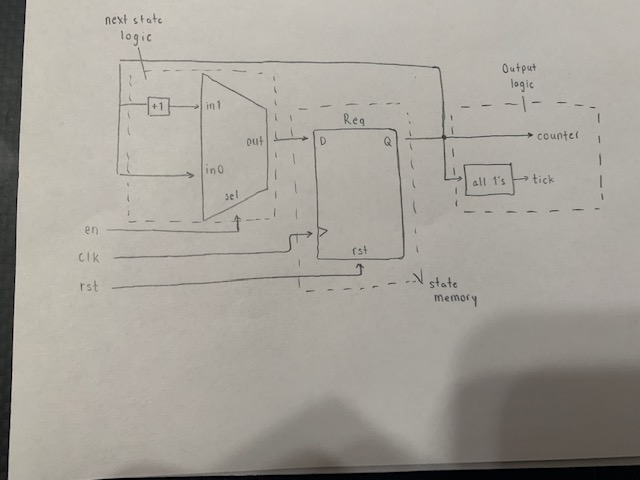
\includegraphics[width=.85\textwidth,angle=0,origin=c]{Counter}
		\caption{Counter Diagram for Question 2}
		\label{fig:sim_with_table}
		
	\end{figure}
	
	\item \textbf{If instead of a counter, you wanted to make a shift register that moved the input bits from right to left (low to high). What would you put on the line Q next = /*???*/?}
	
	Q next = Q reg - 1
	
\end{enumerate}

\section*{Code}

\begin{lstlisting}[style=Verilog,
caption=Counter Code,
label=code:ex 
]
`timescale 1ns / 1ps
// Sebastian Lopez ELC 2137 , 2020 -04 -02

module counter #(parameter N = 1)(
input clk , rst , en ,
output [N -1:0]  count ,
output  tick    
);

reg [N -1:0]  Q_reg , Q_next;

always @(posedge clk , posedge  rst)
begin
if (rst)
Q_reg <= 0; 
else 
Q_reg <= Q_next; 
end 

always @*
begin 
if (en)
Q_next = Q_reg + 1; 
else
Q_next = Q_reg; 
end 

assign count = Q_reg; 
assign tick = (Q_reg == {N{1'b1}}) ? 1'b1 : 1'b0; 

endmodule //counter
\end{lstlisting}

\begin{lstlisting}[style=Verilog,
caption=sseg4TDM Code,
label=code:ex 
]
`timescale 1ns / 1ps
// Sebastian Lopez ELC 2137 , 2020 -04 -02

module sseg4_TDM(
input [15:0] data, 
input hex_dec, sign, 
input reset, 
input clock, 
output [6:0] seg, 
output dp, 
output [3:0] an
);

wire [15:0] ebout, mux2out; 
wire [3:0] mux4out; 
wire [6:0] decout; 
wire andecout; 
wire m2sel; 
wire [1:0] digit_sel; 
wire tickout; 

counter #(.N(18)) c1(.clk(clock), .rst(reset), .en(1), .tick(tickout));

counter #(.N(18)) c2(.clk(clock), .en(tickout), .count(digit_sel), .rst(reset));

BCD11 e0(.in(data[10:0]), .out(ebout)); 

mux2 #(.N(16)) mux2A(.in0(data), .in1(ebout), .sel(hex_dec), .out(mux2out)); 

mux4 #(.N(4)) mux4A(.in0(mux2out[3:0]), .in1(mux2out[7:4]), .in2(mux2out[11:8]), .in3(mux2out[15:12]), .sel(digit_sel), .out(mux4out)); 

sseg_decoder s1(.num(mux4out), .sseg(decout)); 

an_decoder an1(.in(digit_sel), .out(an)); 

assign m2sel = ~an[3]; 

and agate1(andecout, sign, m2sel); 

mux2 #(.N(7)) mux2B(.in0(decout), .in1(7'b01111111), .sel(andecout), .out(seg)); 

assign dp = 1; 

endmodule
\end{lstlisting}

\begin{lstlisting}[style=Verilog,
caption=Calculator Code,
label=code:ex 
]
`timescale 1ns / 1ps
// Sebastian Lopez ELC 2137 , 2020 -04 -02

module calc_lab10(
input btnC, btnD, btnU, clock, reset, dp, an, 
input [15:0] sw, 
output [15:0] led, 
output [6:0] seg
);

top_lab9 calc_unit(.sw(sw[11:0]), .btnC(btnC), .btnD(btnD), .btnU(btnU), .clk(clock), .led(led));

sseg4_TDM disp_unit(.data({led[15:0], 8'b00000000}), .hex_dec(sw[15]), 
.sign(sw[14]), .reset(btnC), .clock(clock), .seg(seg), .dp(dp), .an(an)); 

endmodule
\end{lstlisting}

\begin{lstlisting}[style=Verilog,
caption=Counter test Code,
label=code:ex 
]

\end{lstlisting}

\section*{Results}

\begin{figure}[ht]\centering
	
	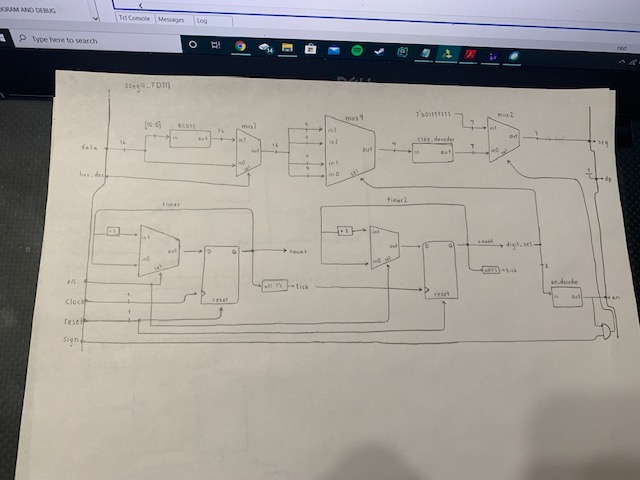
\includegraphics[width=1\textwidth,angle=0,origin=c]{sseg4_TDM}
	\caption{sseg4TDM Diagram}
	\label{fig:sim_with_table}
	
\end{figure}

\begin{figure}[ht]\centering	
	
	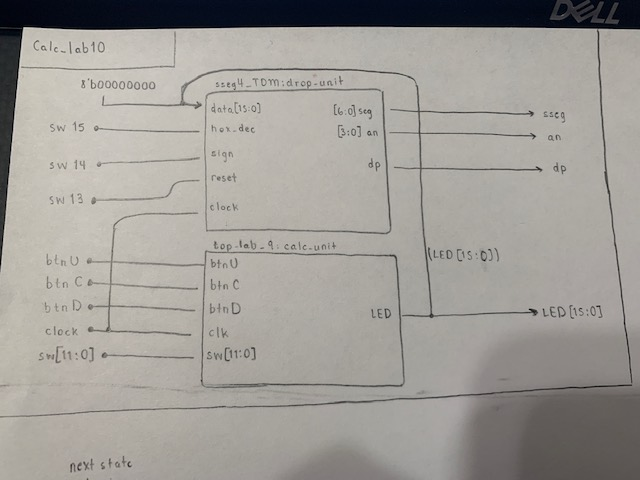
\includegraphics[width=1\textwidth,angle=0,origin=c]{Calculator}
	\caption{Calculator Diagram}
	\label{fig:sim_with_table}
\end{figure}

\begin{figure}[ht]\centering	
	
	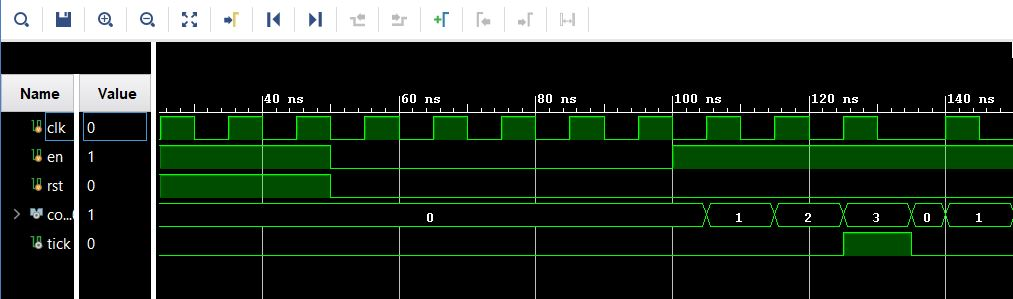
\includegraphics[width=1\textwidth,angle=0,origin=c]{Counter Waveform}
	\caption{Counter Waveform}
	\label{fig:sim_with_table}
\end{figure}

\end{document}
